\chapter{Introduction}\labch{intro}
In the field of formal semantics, pinning down the exact nature of the meaning of conditionals has been a long-standing and controversial topic. Our earliest sources on the meaning of conditionals date back to ancient Greece, where Philo the Dialectician, in a debate with his teacher Diodorus Cronus, argued that a conditional is true exactly when it is not the case that the antecedent is true and the consequent is false, as reported by Sextus Empiricus in the second century of the Common Era \parencite{Kneale1962}. This definition gave rise to the analysis of conditionals in \textcite{Frege1879} and \citepos{Whitehead1910} two-valued propositional framework that modern philosophisers refer to as the \enquote{material conditional}, as defined in \refdef{material}.
\pex
$\intension[w,g]{If $\phi$, $\psi$}=\textiff\phi\supset\psi$\\
\phantom{$\intension[w,g]{If $\phi$, $\psi$}=~$}$\textiff\phi\rightarrow\psi$\\
\phantom{$\intension[w,g]{If $\phi$, $\psi$}=~$}$\textiff\neg\phi\lor\psi$\\
\phantom{$\intension[w,g]{If $\phi$, $\psi$}=~$}$\textiff\phi\land\neg\psi$\labdef{material}
\xe
But, as already noted by \textcite{Frege1879} himself, this definition is woefully inadequate when trying to define the meaning of natural language conditionals, as it leads to a number of highly unintuitive properties that are collectively known as the paradoxes of material implication. One of the gravest of these shortcomings is typically considered to be that this model predicts all conditionals to be true so long as their antecedents are false, irrespective of their actual propositional content \parencite{Lewis1912}.

\section{Strict Semantics}
To rectify this issue, providing a first step towards an intensional treatment of conditionals, \textcite[p.~33]{Peirce1896} and \textcite{Lewis1912,Lewis1914,Lewis1918} proposed an analysis of conditionals where the material conditional must not only be true but necessarily true; i.e., the material implication must be true in all (accessible) possible worlds. This approach is referred to as the strict approach to conditional semantics. Using \citepos{Kripke1963} modal logic semantics, \citepos{Lewis1912,Lewis1914,Lewis1918} definition may be expressed as shown in \refex{strict-intro}.
\ex\label{ex:strict-intro}
$\intension[w,g]{If $\phi$, $\psi$.}=\textiff\square(\phi\supset\psi)$
\xe
This definition successfuly avoids the aforementioned paradox of material implication: Even if the antecedent is false in the actual world, we would still have to evaluate whether the material implication is also true in all possible worlds, including worlds where the antecedent is true.

However, whilst being a definite improvement over the material conditional, this traditional strict conditional semantics still carries a number of issues that preclude it from being considered a real candidate for an accurate semantics of natural language conditionals. One of these issues, for example, relates to the fact that \citepos{Lewis1912,Lewis1914,Lewis1918} semantics would predict that conditionals are transitive by nature (i.e., when \enquote{If $\phi$, $\psi$} and \enquote{If $\psi$, $\chi$} are true, then we would expect \enquote{If $\phi$, $\chi$} to be true as well). Natural language conditionals are not, however, universally transitive by nature, as demonstrated by \refex{transitive}.
\ex
If Brown wins the election, Smith will retire to private life. If Smith dies before the election, Brown will win it. \#Therefore, if Smith dies before the election, then he will retire to private life.\hfill\parencite[p.~166]{Adams1965}\labex{transitive}
\xe
Another issue is that of monotonicity. \textcite{Lewis1912,Lewis1914,Lewis1918} would predict that all conditional antecedents are purely downward monotone with regards to all possible worlds. This has two consequences of note: one positive and one negative. 

The positive consequence of note would be that so-called weak negative polarity items would be licensed in the antecedent of conditionals according to their classical environment-/monotonicity-based licensing theory. Weak negative polarity items, such as \textit{any} or \textit{ever}, are words which are restricted in their distribution to certain contexts (most of which are perceived to be negative by nature). Their classical licensing theory posits that they may only ever occur in downward monotone environments \parencite{Ladusaw1980,Fauconnier1975a,Fauconnier1975b}. 
\ex\label{def:dm-intro}%
\extitle{Downward Monotonicity}%
$f\in D_{\langle\sigma,\tau\rangle}$ is downward monotone iff for all $x,y\in D_\sigma$ s.t. $x\subseteq y$: $f(y)\Rightarrow f(x)$.%

\xe
However, empirical data shows that negative polarity items also occur in the antecedent of conditionals:
\ex
If John had read any book, he would've passed the test.\labex{npi-conditional-good-any-intro}
\xe
Since the strict approach to conditionals would render the antecedent of conditionals downward monotone by nature, this model would correctly predict that negative polarity items are licensed in this environment.

The negative consequence of this presumed downward monotonicity, on the other hand, would be as follows: If we have a conditional that was evaluated to be true, any and all conditionals whose antecedents are mere specifications of the original antecedent must necessarily also be true with respect to the original consequent. However, as noted by \textcite[p.~10]{Lewis1973}, this is clearly not the case for all conditionals. In fact, \textcite{Lewis1973} noted that any conditional \enquote{If $\phi$, $\chi$} may have its antecedent further specified by some proposition $\psi$ such that it leads to the negation of the consequent, yielding a conditional along the lines of \enquote{If $\phi\land\psi$, $\neg\chi$}. In addition, the latter may follow the former in a sequence of conditionals without any feeling of contradiction of infelicity. This is shown in \refex{SS-nuclear-intro}.
\ex\labex{SS-nuclear-intro}If the USA threw its weapons into the sea tomorrow, there would be war;\linebreak but if the USA and the other nuclear powers all threw their weapons into the sea tomorrow, there would be peace.\hfill\parencite[p.~10]{Lewis1973}
\xe
Because the first verifiable mention of such conditional sequences in modern science was done by \textcite{Sobel1970}, such sentences are referred to as \textit{Sobel sequences}.
\ex\labdef{SS-intro}\extitle{Sobel Sequence}A Sobel sequence is any sequence of conditionals that adheres to the pattern of \enquote{If $\phi$, $\chi$; [but] if $(\phi\land\psi)$, $\neg\chi$}, where $\phi\neq\psi$.%
\xe
Since the strict conditional semantics assumes that conditional antecedents are downward monotone by nature, we would erroneously predict all Sobel sequences to be contradictory and, therefore, to be infelicitous. This was one of the main motivations behind the development of the so-called variably-strict approach to conditional semantics \parencite{Stalnaker1968,Lewis1973}.


\section{Variably-Strict Semantics}
\textcite{Stalnaker1968} and \textcite{Lewis1973} introduced the notion that at least subjunctive conditionals (e.g., counterfactuals) do not simply quantify over all accessible worlds but merely over a subset of these worlds. More specifically, they quantify only over those possible worlds that fulfil the requirements of the antecedent and that can be considered the least different to the world that the conditional was uttered in (referred to as the evaluation world, which typically though not necessarily coincides with the actual world $w_0$). To achieve this, researchers have introduced the concepts of world similarity as well as world closeness. These terms were often used nigh interchangeably until relatively recently. To differentiate, world closeness refers to ranking each possible world in relation to a specific evaluation world according to some metric, and this metric is typically equal to world similarity (though not necessarily). World similarity, in turn, measures how similar any given possible world should be considered to the evaluation world, and was nigh-simultaneously developed by \textcite{Stalnaker1968}, \textcite{Stalnaker1970}, \textcite{Sprigge1970}, \textcite{Lewis1973}, and \textcite{Nute1975}, but first formulated as a notion by \textcite[p.~107]{Todd1964}:
\begin{displayquote}
When we allow for the possibility of the antecedent’s being true in the case of a counterfactual, we are hypothetically substituting a different world for the actual one. It has to be supposed that this hypothetical world is as much like the actual one as possible so that we will have grounds for saying that the consequent would be realised in such a world.
\end{displayquote}
To this end, \textcite{Lewis1973} counts any additional deviation from the evaluation world as a singular decrease in world similarity.\footnote{This view on similarity leads to a number of problems down the line. A more sensible approach concerning how world similarity is to be measured is introduced in \refsec{css-bennett-explanation} and reflects the work of \textcite{Bennett2003} and \textcite{Arregui2009}.} This similarity ordering is traditionally visually represented by concentric layers, where each layer further out represents an additional decrease in similarity to the evaluation world, which is found at the very centre, as seen in \reffig{similarity-ordering-intro}.
\begin{figure}[!htb]
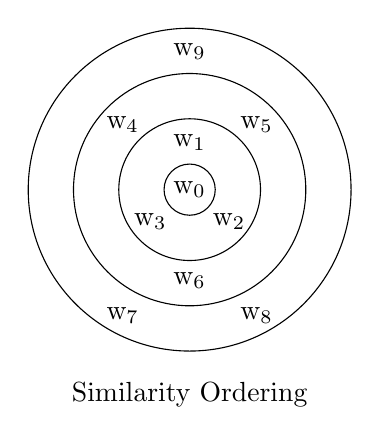
\begin{tikzpicture}
	\coordinate (O) at (0,0);

	\draw[fill=white] (O) circle (2.05);
	\draw[fill=white] (O) circle (1.475);
	\draw[fill=white] (O) circle (0.9);
	\draw[fill=white] (O) circle (0.325)node {w$_0$};

	\node at (0,0.6) {w$_1$};
	\node at (0.5,-0.4) {w$_2$};
	\node at (-0.5,-0.4) {w$_3$};
	
	\node at (-0.85,0.825) {w$_4$};
	\node at (0.85,0.825) {w$_5$};
	\node at (0,-1.15) {w$_6$};
	
	\node at (-0.85,-1.6) {w$_7$};
	\node at (0.85,-1.6) {w$_8$};
	\node at (0,1.75) {w$_9$};
	
	\node at (0,-2.6) {Similarity Ordering};
\end{tikzpicture}
\caption{Similarity ordering with respect to the evaluation world $w_0$, where the worlds $w_{1\leqslant n\leqslant3}$ are equally similar to $w_0$, but more similar to $w_0$ than $w_{4\leqslant n\leqslant9}$, and where $w_{4\leqslant n\leqslant6}$ are still more similar to $w_0$ than $w_{7\leqslant n\leqslant9}$.}
\labfig{similarity-ordering-intro}
\end{figure}

\noindent We therefore define the variably-strict analysis's conditional semantics as in \refdef{variablystrict-intro}:
\ex\labdef{variablystrict-intro}For all contexts $c$, \enquote{If $\phi$, $\psi$} is true at $w$ in $c$ iff all the closest $\phi$-worlds to $w$ are $\psi$-worlds, where closeness is determined by similarity.%
\xe
Alternatively, the same underlying mechanism can be expressed in a more formalised fashion as shown in \refdef{variablystrictformal-intro}, where the accessibility function $f_\leqslant(p,w)$ returns the set of the $p$-worlds that are closest to the evaluation world $w$.\enlargethispage*{1.5\baselineskip}
\ex\labdef{variablystrictformal-intro}$\intension{If $\phi$, $\psi$}=[\lambda w_s.\forall v:v\in f_\leqslant([\lambda w'_s.\phi(w')],w)[\psi(v)]]$\xe\newpage
\noindent This effectively renders conditionals non-monotonic in their domain of quantification. 
\ex\label{def:nm-intro}%
\extitle{Non-Monotonicity}%
$f\in D_{\langle\sigma,\tau\rangle}$ is non-monotone iff for all $x,y\in D_\sigma$ s.t. $x\subseteq y$:\\$f(y)\not\Rightarrow f(x)$ and $f(x)\not\Rightarrow f(y)$.%

\xe
This has, again, one negative and one positive consequence of note.

For the licensing of negative polarity items in the antecedent of conditionals, the presumed non-monotone nature of conditional antecedents would entail that no weak negative polarity items should be licensed in this environment according to \textcite{Fauconnier1975a,Fauconnier1975b} and \citepos{Ladusaw1980} licensing theory. This is an obviously wrong prediction, given the empirical data shown in \refex{npi-conditional-good-any-intro}.

For Sobel sequences, on the other hand, the result would be a bit more positive. Given the non-monotone nature of antecedents, the $\phi$-conditional no longer considers the worlds of the $\phi\land\psi$-conditional for its own evaluation. Instead, the two conditionals quantify over two completely separate sets of worlds, as illustrated in \reffig{stalnakerlewis-SS-intro}.
\begin{figure}[!htb]
    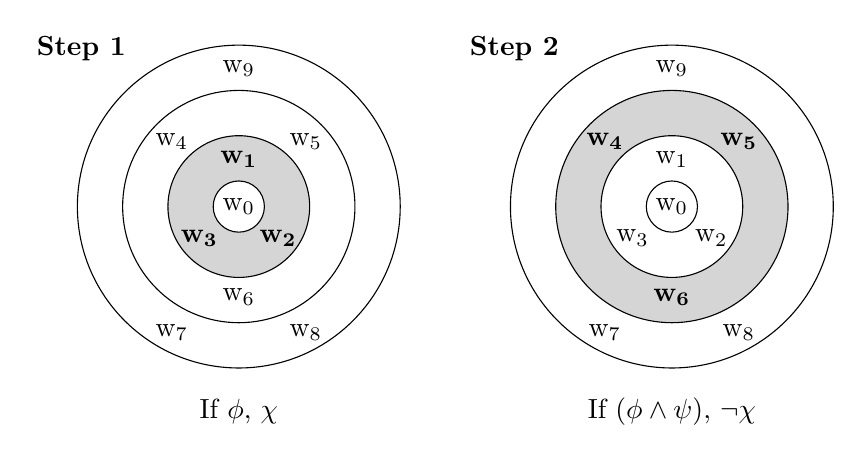
\begin{tikzpicture}
	\coordinate (O) at (0,0);
    \node at (-2,2) {\textbf{Step 1}};
	\draw[fill=white] (O) circle (2.05);
	\draw[fill=white] (O) circle (1.475);
	\draw[fill=gray!33] (O) circle (0.9);
	\draw[fill=white] (O) circle (0.325)node {w\textsubscript{0}};

	\node at (0,0.6) {\textbf{w\textsubscript{1}}};
	\node at (0.5,-0.4) {\textbf{w\textsubscript{2}}};
	\node at (-0.5,-0.4) {\textbf{w\textsubscript{3}}};
	
	\node at (-0.85,0.825) {w\textsubscript{4}};
	\node at (0.85,0.825) {w\textsubscript{5}};
	\node at (0,-1.15) {w\textsubscript{6}};
	
	\node at (-0.85,-1.6) {w\textsubscript{7}};
	\node at (0.85,-1.6) {w\textsubscript{8}};
	\node at (0,1.75) {w\textsubscript{9}};
	
	\node at (0,-2.6) {If $\phi$, $\chi$};
	
	
	\begin{scope}[xshift=5.5cm]
		\coordinate (O) at (0,0);
        \node at (-2,2) {\textbf{Step 2}};
    \draw[fill=white] (O) circle (2.05);
	\draw[fill=gray!33] (O) circle (1.475);
	\draw[fill=white] (O) circle (0.9);
	\draw[fill=white] (O) circle (0.325)node {w\textsubscript{0}};

	\node at (0,0.6) {w\textsubscript{1}};
	\node at (0.5,-0.4) {w\textsubscript{2}};
	\node at (-0.5,-0.4) {w\textsubscript{3}};
	
	\node at (-0.85,0.825) {\textbf{w\textsubscript{4}}};
	\node at (0.85,0.825) {\textbf{w\textsubscript{5}}};
	\node at (0,-1.15) {\textbf{w\textsubscript{6}}};
	
	\node at (-0.85,-1.6) {w\textsubscript{7}};
	\node at (0.85,-1.6) {w\textsubscript{8}};
	\node at (0,1.75) {w\textsubscript{9}};
	
	\node at (0,-2.6) {If $(\phi\land\psi)$, $\neg\chi$};
	\end{scope}
\end{tikzpicture}
\caption{Domains of quantification for Sobel sequences according to \textcite{Stalnaker1968} and \citepos{Lewis1973} variably-strict conditional analyses. For all $w_n$-worlds: If $n\geqslant1$, then $\phi=1$ is true for $w_n$, and if $n\geqslant 4$, then $\psi=1$ holds true for $w_n$. If $n\geqslant 7$, then some proposition $\omega=1$ such that $\omega\neq\phi$, $\omega\neq\psi$, and $\phi,\psi$ do not precede $\omega$ on some causal chain of events.}
\labfig{stalnakerlewis-SS-intro}
\end{figure}

\noindent Therefore, no conflicting statement is made, rendering Sobel sequences felicitous.

Crucially, the order of the conditionals should be of no further relevance because the set of the closest $\phi$-worlds and the set of the closest $\phi\land\psi$-worlds are disjoint. This does not, however, appear to not be the case: Reverse Sobel sequences---defined in \refdef{rSS-intro}---have traditionally been observed to be infelicitous, even though they, as the name would imply, consist of the same conditionals as a Sobel sequence, merely in reverse order. The infelicity of such sequences is typically demonstrated with the counterpart to \refex{SS-nuclear-intro}, as seen in \refex{rSS-nuclear-intro}, that was originally provided by \textcite{Heim1994}.
\ex\labdef{rSS-intro}\extitle{Reverse Sobel Sequence}A reverse Sobel sequence is any sequence of conditionals that adheres to the pattern of \enquote{If $(\phi\land\psi)$, $\neg\chi$; [but] if $\phi$, $\chi$}, where $\phi\neq\psi$.%
\xe
\ex\labex{rSS-nuclear-intro}If the USA and the other nuclear powers all threw their weapons into the sea tomorrow, there would be peace;\\\ljudge\# but if the USA threw its weapons into the sea tomorrow, there would be war.\\\emptyfill\parencite{Heim1994}
\xe

The hereto illustrated variably-strict conditional analysis fails to predict the infelicity or perceived inconsistency of the reverse Sobel sequence, as the domains of quantification remain entirely disjoint, as seen in \reffig{stalnakerlewis-rSS-intro}:
\begin{figure}[!htb]
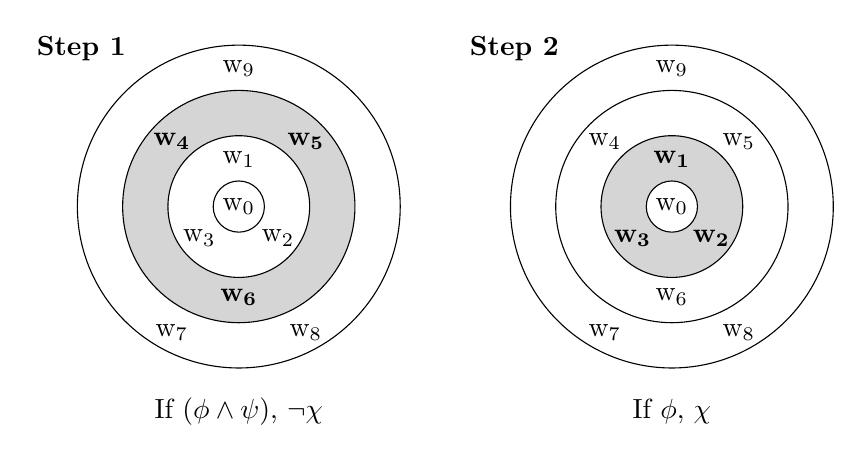
\begin{tikzpicture}
	\coordinate (O) at (0,0);
    \node at (-2,2) {\textbf{Step 1}};
	\draw[fill=white] (O) circle (2.05);
	\draw[fill=gray!33] (O) circle (1.475);
	\draw[fill=white] (O) circle (0.9);
	\draw[fill=white] (O) circle (0.325)node {w\textsubscript{0}};

	\node at (0,0.6) {w\textsubscript{1}};
	\node at (0.5,-0.4) {w\textsubscript{2}};
	\node at (-0.5,-0.4) {w\textsubscript{3}};
	
	\node at (-0.85,0.825) {\textbf{w\textsubscript{4}}};
	\node at (0.85,0.825) {\textbf{w\textsubscript{5}}};
	\node at (0,-1.15) {\textbf{w\textsubscript{6}}};
	
	\node at (-0.85,-1.6) {w\textsubscript{7}};
	\node at (0.85,-1.6) {w\textsubscript{8}};
	\node at (0,1.75) {w\textsubscript{9}};
	
	\node at (0,-2.6) {If $(\phi\land\psi)$, $\neg\chi$};
	
	
	\begin{scope}[xshift=5.5cm]
		\coordinate (O) at (0,0);
        \node at (-2,2) {\textbf{Step 2}};
    \draw[fill=white] (O) circle (2.05);
	\draw[fill=white] (O) circle (1.475);
	\draw[fill=gray!33] (O) circle (0.9);
	\draw[fill=white] (O) circle (0.325)node {w\textsubscript{0}};

	\node at (0,0.6) {\textbf{w\textsubscript{1}}};
	\node at (0.5,-0.4) {\textbf{w\textsubscript{2}}};
	\node at (-0.5,-0.4) {\textbf{w\textsubscript{3}}};
	
	\node at (-0.85,0.825) {w\textsubscript{4}};
	\node at (0.85,0.825) {w\textsubscript{5}};
	\node at (0,-1.15) {w\textsubscript{6}};
	
	\node at (-0.85,-1.6) {w\textsubscript{7}};
	\node at (0.85,-1.6) {w\textsubscript{8}};
	\node at (0,1.75) {w\textsubscript{9}};
	
	\node at (0,-2.6) {If $\phi$, $\chi$};
	\end{scope}
\end{tikzpicture}%
\caption{Quantificational domains for reverse Sobel sequences according to \textcite{Stalnaker1968} and \citepos{Lewis1973} variably-strict conditional analyses. For all worlds $w_n$: If $n\geqslant1$, then $\phi=1$ is true for $w_n$, and if $n\geqslant 4$, then $\psi=1$ holds true for $w_n$. If $n\geqslant 7$, then some proposition $\omega=1$ such that $\omega\neq\phi$, $\omega\neq\psi$, and $\phi,\psi$ do not precede $\omega$ on some causal chain of events.}\labfig{stalnakerlewis-rSS-intro}
\end{figure}

\noindent Since the sequence's two relevant domains of quantification are entirely disjoint, it makes---from a semantic point of view---no difference in which order a claim about the respective worlds is made. As such, the variably-strict semantics would falsely predict all reverse Sobel sequences to be felicitous.\vfill
\section{(Semi-)Dynamic Strict Semantics}
The infelicity of reverse Sobel sequences led to a renewed interest in the strict conditional analysis, as that approach correctly predicted the infelicity of reverse Sobel sequences. To account for regularly ordered Sobel sequences, however, the original model requires additional constraints on the domain of quantification, such that Sobel sequences do not yield a contradiction---without affecting the fact that reverse Sobel sequences do. This led to the inception of the (semi-)dynamic strict conditional line of thought, as originally put forth by \textcite{Fintel2001} and \textcite{Gillies2007}. 

\textcite{Fintel2001} proposes that counterfactual conditionals are analysed as strict conditionals that apply to a contextually determined domain of quantification. Counterfactual conditionals also carry a presupposition of entertainability, which means that their antecedents must be possible with respect to the aforementioned contextually defined domain of quantification. If this presupposition is violated---that is, the contextually determined domain of quantification does not contain any antecedent world---then the contextual domain of quantification is expanded to include all possible worlds up to and including the closest possible antecedent worlds. For this reason, \textcite{Fintel2001} also refers to the contextually-expanding domain of quantification as a modal horizon. This operation is formally executed through the accessibility relation $f_\sigma$ as specified by the context $\sigma$ (which initially comprises only the evaluation world itself). If the context lacks any valid antecedent worlds, the respective counterfactual modifies $\sigma$ to include all worlds up to and including the closest antecedent worlds. The modified context is then maintained for any subsequent counterfactual conditionals, with the process of modifying $\sigma$ being repeated as necessary (i.e., whenever no valid antecedent world already exists in the modal horizon).\linebreak\newpage\noindent This entire process in formally defined in its entirety in \refdef{fintel-intro}.
\pex\labdef{fintel-intro}\resizebox{395pt}{!}{\pextitle{Modal Horizon and Counterfactual Semantics by \citet{Fintel2001} for `If p, q'}}
\a\extitle{Context Change Potential}$f_\sigma+\intension[]{would}_{KvF}(q)(p)(w) = f^p_\sigma = [\lambda w_s.f_\sigma(w)\cup\{w':\forall w''\in p[w'\leqslant_w w'']\}]$
\a\extitle{Truth Conditions}$\intension[\sigma]{would}_{KvF}=[\lambda q_{<s,t>}.[\lambda p_{<s,t>}.[\lambda w_s.\hspace{1mm}\forall v\in f^p_\sigma(w)\cap p\hspace{0.5mm}[q(v)]\hspace{1mm}]]]$
\xe
This process is illustrated in \reffig{fintel-contextchange-intro} for the conditional \enquote{If p, q}:
\begin{figure}[!htb]
\resizebox{\textwidth}{!}{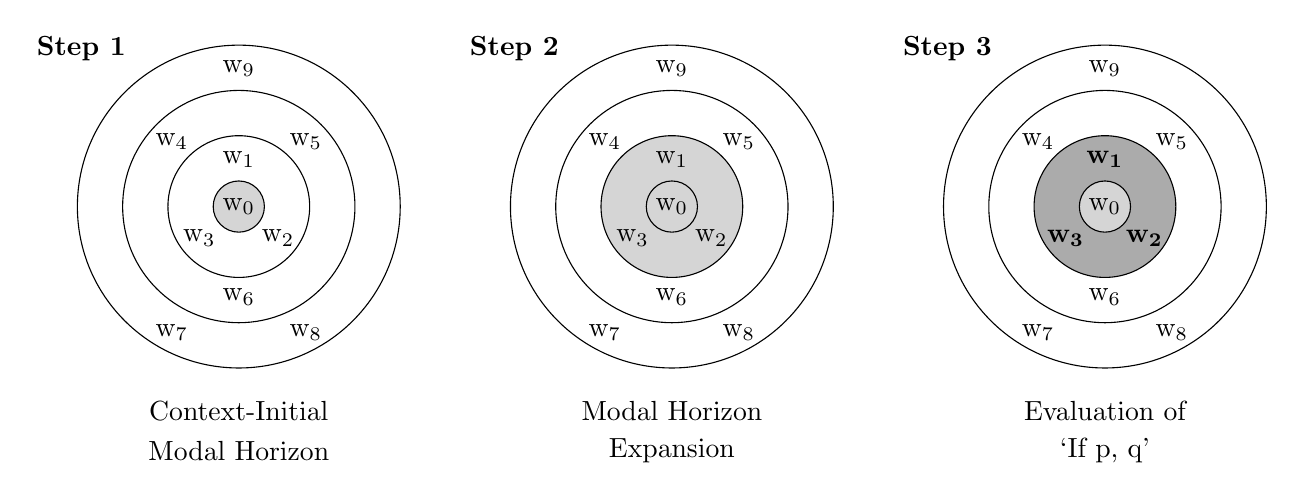
\begin{tikzpicture}
	\coordinate (O) at (0,0);
    \node at (-2,2) {\textbf{Step 1}};
	\draw[fill=white] (O) circle (2.05);
	\draw[fill=white] (O) circle (1.475);
	\draw[fill=white] (O) circle (0.9);
	\draw[fill=gray!33] (O) circle (0.325)node {w\textsubscript{0}};

	\node at (0,0.6) {w\textsubscript{1}};
	\node at (0.5,-0.4) {w\textsubscript{2}};
	\node at (-0.5,-0.4) {w\textsubscript{3}};
	
	\node at (-0.85,0.825) {w\textsubscript{4}};
	\node at (0.85,0.825) {w\textsubscript{5}};
	\node at (0,-1.15) {w\textsubscript{6}};
	
	\node at (-0.85,-1.6) {w\textsubscript{7}};
	\node at (0.85,-1.6) {w\textsubscript{8}};
	\node at (0,1.75) {w\textsubscript{9}};
	
	\node at (0,-2.6) {Context-Initial};
	\node at (0,-3.1) {Modal Horizon};
	
	
	\begin{scope}[xshift=5.5cm]
		\coordinate (O) at (0,0);
        \node at (-2,2) {\textbf{Step 2}};
    \draw[fill=white] (O) circle (2.05);
	\draw[fill=white] (O) circle (1.475);
	\draw[fill=gray!33] (O) circle (0.9);
	\draw[fill=gray!33] (O) circle (0.325)node {w\textsubscript{0}};

	\node at (0,0.6) {w\textsubscript{1}};
	\node at (0.5,-0.4) {w\textsubscript{2}};
	\node at (-0.5,-0.4) {w\textsubscript{3}};
	
	\node at (-0.85,0.825) {w\textsubscript{4}};
	\node at (0.85,0.825) {w\textsubscript{5}};
	\node at (0,-1.15) {w\textsubscript{6}};
	
	\node at (-0.85,-1.6) {w\textsubscript{7}};
	\node at (0.85,-1.6) {w\textsubscript{8}};
	\node at (0,1.75) {w\textsubscript{9}};
	
	\node at (0,-2.6) {Modal Horizon};
	\node at (0,-3.1) {Expansion};
	
	
	\begin{scope}[xshift=5.5cm]
		\coordinate (O) at (0,0);
        \node at (-2,2) {\textbf{Step 3}};
    \draw[fill=white] (O) circle (2.05);
	\draw[fill=white] (O) circle (1.475);
	\draw[fill=gray!66] (O) circle (0.9);
	\draw[fill=gray!33] (O) circle (0.325)node {w\textsubscript{0}};

	\node at (0,0.6) {\textbf{w\textsubscript{1}}};
	\node at (0.5,-0.4) {\textbf{w\textsubscript{2}}};
	\node at (-0.5,-0.4) {\textbf{w\textsubscript{3}}};
	
	\node at (-0.85,0.825) {w\textsubscript{4}};
	\node at (0.85,0.825) {w\textsubscript{5}};
	\node at (0,-1.15) {w\textsubscript{6}};
	
	\node at (-0.85,-1.6) {w\textsubscript{7}};
	\node at (0.85,-1.6) {w\textsubscript{8}};
	\node at (0,1.75) {w\textsubscript{9}};
	
	\node at (0,-2.6) {Evaluation of};
	\node at (0,-3.1) {`If p, q'};
	\end{scope}
	\end{scope}
	
\end{tikzpicture}}
\caption{Modal horizon (all shades of grey) and antecedent worlds quantified over (dark grey) for the conditional `If p, q', according to \citepos{Fintel2001} semi-dynamic strict analysis, when the context initial modal horizon does not contain any suitable antecedent worlds. For all worlds $w_n$: If $n\geqslant1$, then $p=1$ is true for $w_n$.}\labfig{fintel-contextchange-intro}
\end{figure}

For Sobel sequences, this means that the $\phi$-conditional updates $\sigma$ such that it contains all possible worlds up to including the closet $\phi$-worlds. Crucially, this means that the modal horizon does not contain any $\phi\land\psi$-worlds, since these worlds are less close to the evaluation world than the closet $\phi$-worlds. Since the $\phi\land\psi$-conditional's domain of quantification would then be empty, it further updates $\sigma$ to include the closest $\phi\land\psi$-worlds as as well. This way, the felicity of Sobel sequences would be explained, as illustrated in \reffig{fintel-SS-intro}.\pagebreak
\begin{figure}[!htb]
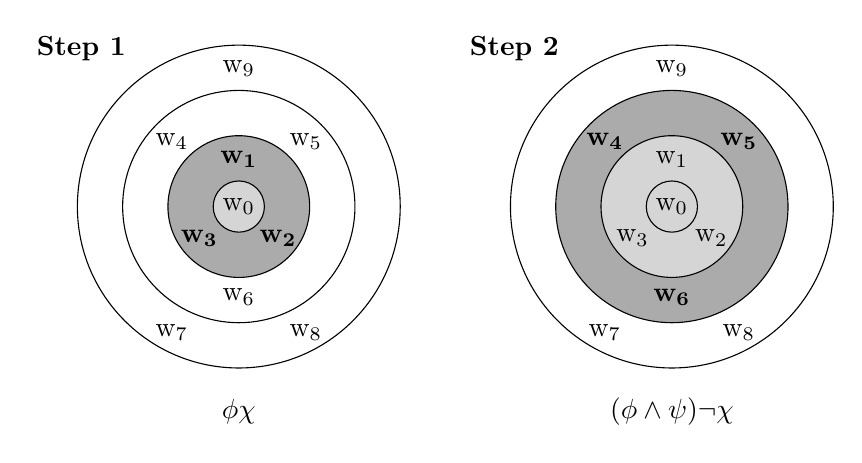
\begin{tikzpicture}
	\coordinate (O) at (0,0);
    \node at (-2,2) {\textbf{Step 1}};
	\draw[fill=white] (O) circle (2.05);
	\draw[fill=white] (O) circle (1.475);
	\draw[fill=gray!66] (O) circle (0.9);
	\draw[fill=gray!33] (O) circle (0.325)node {w\textsubscript{0}};

	\node at (0,0.6) {\textbf{w\textsubscript{1}}};
	\node at (0.5,-0.4) {\textbf{w\textsubscript{2}}};
	\node at (-0.5,-0.4) {\textbf{w\textsubscript{3}}};
	
	\node at (-0.85,0.825) {w\textsubscript{4}};
	\node at (0.85,0.825) {w\textsubscript{5}};
	\node at (0,-1.15) {w\textsubscript{6}};
	
	\node at (-0.85,-1.6) {w\textsubscript{7}};
	\node at (0.85,-1.6) {w\textsubscript{8}};
	\node at (0,1.75) {w\textsubscript{9}};
	
	\node at (0,-2.6) {$\phi\cf\chi$};
	
	
	\begin{scope}[xshift=5.5cm]
		\coordinate (O) at (0,0);
        \node at (-2,2) {\textbf{Step 2}};
    \draw[fill=white] (O) circle (2.05);
	\draw[fill=gray!66] (O) circle (1.475);
	\draw[fill=gray!33] (O) circle (0.9);
	\draw[fill=gray!33] (O) circle (0.325)node {w\textsubscript{0}};

	\node at (0,0.6) {{w\textsubscript{1}}};
	\node at (0.5,-0.4) {{w\textsubscript{2}}};
	\node at (-0.5,-0.4) {{w\textsubscript{3}}};
	
	\node at (-0.85,0.825) {\textbf{w\textsubscript{4}}};
	\node at (0.85,0.825) {\textbf{w\textsubscript{5}}};
	\node at (0,-1.15) {\textbf{w\textsubscript{6}}};
	
	\node at (-0.85,-1.6) {w\textsubscript{7}};
	\node at (0.85,-1.6) {w\textsubscript{8}};
	\node at (0,1.75) {w\textsubscript{9}};
	
	\node at (0,-2.6) {$(\phi\land\psi)\cf\neg\chi$};
	\end{scope}
\end{tikzpicture}
\caption{Quantificational domains for Sobel sequences according to \citepos{Fintel2001} semi-dynamic strict conditional analysis. For all worlds $w_n$: If $n\geqslant1$, then $\phi=1$ is true for $w_n$, and if $n\geqslant 4$, then $\psi=1$ holds true for $w_n$. Non-antecedent worlds present within the modal horizon are shaded in the lighter grey.}\labfig{fintel-SS-intro}
\end{figure}

For reverse Sobel sequences, the situation is slightly different. The initial $\phi\land\psi$-conditional update $\sigma$ to include all possible worlds of similarity equal to or greater than the closest $\phi\land\psi$-worlds. Naturally, this also includes the closest $\phi$-worlds. 

\begin{figure}[!htb]
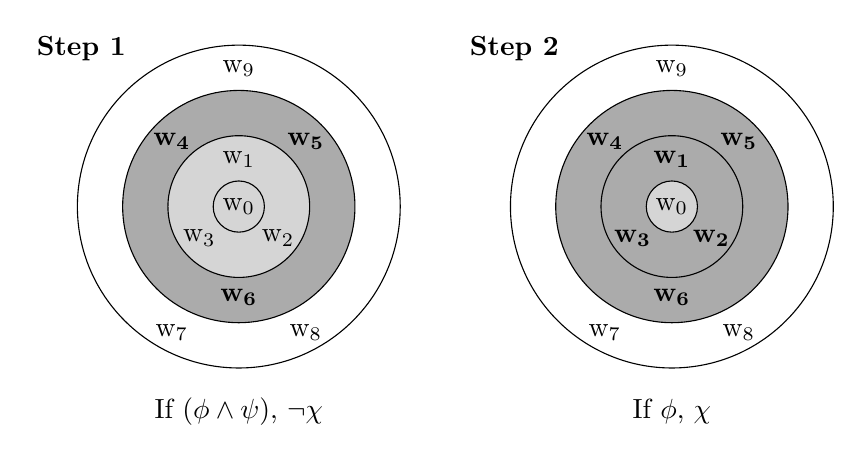
\begin{tikzpicture}
	\coordinate (O) at (0,0);
    \node at (-2,2) {\textbf{Step 1}};
	\draw[fill=white] (O) circle (2.05);
	\draw[fill=gray!66] (O) circle (1.475);
	\draw[fill=gray!33] (O) circle (0.9);
	\draw[fill=gray!33] (O) circle (0.325)node {w\textsubscript{0}};

	\node at (0,0.6) {{w\textsubscript{1}}};
	\node at (0.5,-0.4) {{w\textsubscript{2}}};
	\node at (-0.5,-0.4) {{w\textsubscript{3}}};
	
	\node at (-0.85,0.825) {\textbf{w\textsubscript{4}}};
	\node at (0.85,0.825) {\textbf{w\textsubscript{5}}};
	\node at (0,-1.15) {\textbf{w\textsubscript{6}}};
	
	\node at (-0.85,-1.6) {w\textsubscript{7}};
	\node at (0.85,-1.6) {w\textsubscript{8}};
	\node at (0,1.75) {w\textsubscript{9}};
	
	\node at (0,-2.6) {If $(\phi\land\psi)$, $\neg\chi$};
	
	
	\begin{scope}[xshift=5.5cm]
		\coordinate (O) at (0,0);
        \node at (-2,2) {\textbf{Step 2}};
    \draw[fill=white] (O) circle (2.05);
	\draw[fill=gray!66] (O) circle (1.475);
	\draw[fill=gray!66] (O) circle (0.9);
	\draw[fill=gray!33] (O) circle (0.325)node {w\textsubscript{0}};

	\node at (0,0.6) {\textbf{w\textsubscript{1}}};
	\node at (0.5,-0.4) {\textbf{w\textsubscript{2}}};
	\node at (-0.5,-0.4) {\textbf{w\textsubscript{3}}};
	
	\node at (-0.85,0.825) {\textbf{w\textsubscript{4}}};
	\node at (0.85,0.825) {\textbf{w\textsubscript{5}}};
	\node at (0,-1.15) {\textbf{w\textsubscript{6}}};
	
	\node at (-0.85,-1.6) {w\textsubscript{7}};
	\node at (0.85,-1.6) {w\textsubscript{8}};
	\node at (0,1.75) {w\textsubscript{9}};
	
	\node at (0,-2.6) {If $\phi$, $\chi$};
	\end{scope}
\end{tikzpicture}
\caption{Quantificational domains for reverse Sobel sequences according to \citepos{Fintel2001} semi-dynamic strict conditional analysis. For all worlds $w_n$: If $n\geqslant1$, then $\phi=1$ is true for $w_n$, and if $n\geqslant 4$, then $\psi=1$ holds true for $w_n$. Non-antecedent worlds present within the modal horizon are shaded in the lighter grey.}\labfig{fintel-rSS-intro}
\end{figure}
As illustrated in \reffig{fintel-rSS-intro}, the subsequent $\phi$-conditional's domain of quantification then already contains some antecedent worlds and, as such, does not require an expansion of the modal horizon. Neither does the modal horizon contract to exclude any semantically unnecessary worlds. The $\phi$-conditional would therefore quantify not only over the closest $\phi$-worlds, but any other $\phi$-worlds already present in the context, including the closest $\phi\land\psi$-worlds. This would obviously contradict the meaning of the previous $\phi\land\psi$-conditional, thereby deriving the infelicity of reverse Sobel sequences.


But what are the consequences of this model for negative polarity items? The semantics proposed in \refdef{fintel-intro} would render the antecedent of conditionals to be downward monotone by nature---but only with respect to conditionals that would be defined by its modal horizon. This special type of downward monotonicity has been termed \textit{Strawson downward monotone} and was proposed by \textcite{Fintel1999} to also license negative polarity items (see \refsec{NPI-accounts-mono} for details). As such, the (semi-)dynamic strict approach to conditionals would not only correctly predict Sobel sequences to felicitous, reverse Sobel sequences to be infelicitous, but also negative polarity items to be licensed.


\section{Current Developments}
In recent years, the debate on whether or not conditionals should be modelled in a (semi-)dynamic strict or in a variably-strict manner has resurged in importance. One of the main contributing factors of this resurgence was the discovery of some consistently felicitous reverse Sobel sequences \parencite{Moss2012}, as seen in \refex{moss-intro}.
\pex\label{ex:moss-intro}
\contextpex{Suppose John and Mary are our mutual friends. John was going to ask Mary to marry him, but chickened out at the last minute. I know Mary much better than you do, and you ask me whether Mary might have said yes if John had proposed. I tell you that I swore to Mary that I would never tell anyone that information, which means that strictly speaking, I cannot answer your question. But I say that I will go so far as to tell you two facts:}
\a If John had proposed to Mary and she had said yes, he would have been really happy.
\a But if John had proposed, he would have been really unhappy.\\\emptyfill\parencite[p.~577]{Moss2012}
\xe
As the (semi-)dynamic strict approach would summarily rule out the felicity of \refex{moss-intro}, many semanticists have returned to a variably-strict semantics, as that framework does not intrinsically disallow felicitous reverse Sobel sequences. However, as an extremely large number of reverse Sobel sequences are, in fact, infelicitous, a number of supererogatory pragmatic mechanisms have been proposed in addition to a variably-strict semantics such that they selectively rule out some but not all reverse Sobel sequences \parencite{Moss2012,Klecha2011,Klecha2014,Klecha2015,Lewis2018,Krassnig2017,Krassnig2020}. We refer to \refch{SS} for details.

In addition, the traditionalist monotonicity-/environment-based approach to negative polarity item licensing is gradually being superseded by operator-based approaches \parencite{Lee1994,Lahiri1998,Crnic2011,Crnic2014-dogma,Crnic2014-nm,Jeong2021} that would no longer automatically exclude the possibility of a variably-strict semantics. This development is in large part due to the fact that negative polarity items are sometimes, depending on the context, also licensed in environments that are non-monotone by nature. This is shown, for example, in \refex{nm-intro}.
\pex\label{ex:nm-intro}
\a Exactly four of my students have ever read a book.\label{ex:nm-intro1}
\a \ljudge{\#}Exactly four hundred of my students have ever read a book.\label{ex:nm-intro2}
\xe
For the operator-based approach, one of the most promising avenues is the hypothesis that negative polarity items are actually licensed by a covert \textit{even}-like operator that imposes a scalar probability presupposition upon any statement that wishes to license a negative polarity item. The increase in popularity of such approaches is in large part due to the fact that an environment-based licensing theory would have trouble accounting for why a negative polarity item is licensed in \refex{nm-intro1} but not in \refex{nm-intro2}, as the environment of both sentences should technically be the same (displaying only a difference in number). An operator-based licensing theory, on the other hand, might be able to account for this differences based upon the properties of the licensing operator \parencite[see][]{Crnic2011,Crnic2014-nm}. Not being restricted to a specific kind of monotone environment, both the variably-strict and (semi-)dynamic strict approaches to conditionals may be valid candidates and need to be reevaluated within the framework of such an operator-based licensing theory of negative polarity items to see if either approach has an explanatory advantage over the other.

\section{Aims and Outline of this Dissertation}
The overall aim of this thesis is to contribute to the debate on whether or not conditionals should be modelled in a variably-strict or in a (semi-)dynamic strict manner. We do this by examining the two aforementioned phenomena that provide a window into what is required of an accurate conditional semantics: negative polarity items and (reverse) Sobel sequences. These issues were specifically chosen for their crucial role in the debate between the two conditional approaches. Negative polarity items have long since been thought of to impose restrictions upon the underlying semantics of conditionals, traditionally having required a downward monotone environment. Reverse Sobel sequences and their (in-)felicity distribution, on the other hand, has long since been a confounding factor in the debate that switches forth and back between supporting one approach or the other. As such, finally resolving (i) which factors empirically decide whether or not a reverse Sobel sequence is felicitous or infelicitous and (ii) whether or not the operator-based approach to negative polarity items makes differing predictions with respect to the two conditional theories are perhaps the two most important key aspects in deciding between the two approaches.

For negative polarity items, we explore the two main licensing theories in \refch{npi}: the environment or monotonicity-based approach and the operator or \textit{even}-based approach. There, we examine the distribution of negative polarity items across a wide spectrum of different non-conditional environments and evaluate how well the environment-based approach and the operator-based approach to negative polarity item licensing account for the empirical data shown there. We use the results of this evaluation to decide which of the approaches has an explanatory advantage. In \refch{npi-conditionals}, we then examine the distribution of negative polarity items in conditionals and evaluate how the model chosen in \refch{npi} may account for this data using both a variably-strict and a (semi-)dynamic strict account. We also evaluate if either approach to conditionals can be improved upon to better represent the empirical distribution of negative polarity items in conditional antecedents and, overall, which approach more closely reflects empirical reality when combined with the chosen approach to negative polarity item licensing. We show that, for negative polarity items, the (semi-)dynamic strict approach appears to have an explanatory advantage over the variably-strict approach (albeit a minor one).

We cover reverse Sobel sequences as well as regularly ordered Sobel sequences in \refch{SS}, \refch{pragmatics-SS}, and \refch{ippolito}. First, we examine the disparate examples of reverse Sobel sequences and evaluate which factors might decide reverse Sobel sequence felicity in \refch{SS}. To this end, we discuss and examine factors that were previously proposed in the literature, conduct an experiment to verify some of the claims made in the literature, and finally isolate the key factor in reverse Sobel sequence felicity (as well as a number of highly influential subfactors): namely, contrastive stress. Then, in \refch{pragmatics-SS}, we formalise a pragmatic approach based on the findings of the previous chapter, combine it with both the variably-strict as well as the (semi-)dynamic strict account, and evaluate which of the two conditional semantics is better able to derive the desired empirical distribution when combined with the aforementioned pragmatic mechanism. We show that both approaches to conditionals are equally capable of deriving all of the known associated empirical data. Lastly, in \refch{ippolito}, we evaluate one of the most recent and promising approaches to reverse Sobel sequence (in-)felicity, the one proposed by \textcite{Ippolito2020}, and compare it to the model we have constructed in the preceding chapter.

Finally, in \refch{conclusion}, we summarise all of our findings and evaluate how they impact the debate between the variably-strict approach and the (semi-)dynamic strict approach to conditionals.